\documentclass[12pt]{article}

% --------------------
% Basic Packages
% --------------------
\usepackage[a4paper,margin=1in]{geometry}
\usepackage{setspace}
\usepackage{graphicx}
\usepackage{amsmath}
\usepackage{amssymb}
\usepackage{array}
\usepackage{float}

\onehalfspacing

% --------------------
% Title and Author
% --------------------
\title{Hybrid Machine Learning and Deep Learning Models\\for Robust IoT Cybersecurity}
\author{A.~Jeswin Karunya Benedict}
\date{}

\begin{document}
\maketitle



%=================================================================
\section{Introduction}
%=================================================================

Internet of Things is one of the most significant paradigm shifts in the history of information technology \cite{al2015internet}. Through the connection of physical devices such as home appliances, wearable health trackers, sensors, self-driving cars, and smart cities to exchange information, gather data, and operate independently, IoT has emerged as a critical facilitator for the current digital economy. Recent projections suggest that there will be more than seventy-five billion IoT connections by the end of this decade, which is expected to produce massive amounts of data. Although the interconnectivity of devices offers many benefits in terms of enhancing efficiency, improving healthcare services, monitoring the environment, and increasing public security, it also poses significant cybersecurity risks that require urgent attention.

The existing network security frameworks, which are designed mainly for traditional computing environments comprising powerful computers and servers, do not take into account certain properties inherent in IoT environments \cite{alaba2017internet}. The lack of computational power, memory, and battery life in IoT nodes makes it impossible to rely on heavy encryption algorithms, regular signature database updates, and other computationally demanding security measures. Additionally, there is such great variety of communication protocols, device vendors, firmware, and applications used that it becomes impossible to use an all-in-one security solution. It should also be noted that adversaries are aware of these vulnerabilities and are actively conducting complex attacks against IoT environments, such as recruiting bots into botnets, conducting DDoS attacks, intercepting messages through man-in-the-middle attacks, manipulating firmware, and moving laterally from one network segment to another.

Machine learning has been identified as a potential solution to these security risks, providing capabilities for learning patterns of statistical significance within network traffic data and detecting unusual patterns of activity without prior knowledge of specific attacks \cite{hasan2019attack}. Traditional machine learning techniques such as support vector machines, decision trees, k-nearest neighbors, and random forests have shown impressive success in artificial environments, delivering high levels of classification accuracy using standard benchmark datasets. Nonetheless, these methods frequently fail to account for temporal relationships, hierarchical abstraction of features, and nonlinear interactions associated with modern persistent attacks on IoT networks. On the other hand, deep learning models possess the capability of learning hierarchical abstract representations from raw or lightly preprocessed data, yet they come with their own set of drawbacks like computationally intensive operations, need for substantial labeled training samples, vulnerability to adversarial attacks, and lack of transparency to humans.

Hybrid approaches that intelligently integrate machine learning and deep learning methods offer an appealing compromise and are generating considerable research focus within the cybersecurity domain \cite{zhang2019hybrid}. The combination of these two methodologies through the synergistic utilization of their respective advantages, namely the reliability, speed, and transparency of traditional machine learning algorithms coupled with the expressiveness and ability to extract meaningful features from deep neural networks, has resulted in considerable advancements in intrusion detection efficacy, generalization to novel attacks, and adaptability to low-resource IoT devices.

This research focus area becomes increasingly pertinent as a result of the increased number of attacks targeting the IoT. Specifically, the Mirai attack of 2016 used hundreds of thousands of insecure IoT devices to launch what has been described as one of the most severe instances of distributed denial of service attack, highlighting the potential destruction brought about by IoT infrastructure security vulnerabilities \cite{vishwakarma2020survey}. Variants of this attack include Hajime, IoT Reaper, and BrickerBot, among others, which demonstrate the consistent threat posed by adversaries interested in exploiting IoT technologies. Industrial IoT represents an even more important aspect of this discussion, given that any vulnerability in the form of compromised sensors in power networks, wastewater management systems, or factories could lead to actual physical implications going beyond the virtual environment.

The rest of this paper is structured as follows. Section~2 provides background information and concepts. Section~3 introduces the main methodologies behind hybrid Internet of Things (IoT) security systems. Section~4 examines the comparison of various methods. Section~5 explores key takeaways and implementation instances. Section~6 highlights existing difficulties and unresolved research problems, and Section~7 suggests possible future research paths. Section~8 concludes the paper.


%=================================================================
\section{Background and Conceptual Foundations}
%=================================================================

It is essential to have a grounded understanding of the relationship between IoT and cybersecurity by recognizing the architectural structure of IoT systems as well as the analytical models employed to analyze the intelligent cybersecurity processes. This section presents a discussion on the terminology used throughout this paper.

\subsection{IoT Architecture and Its Security Surface}

In most cases, IoT systems have been classified based on their three-tier architecture, which consists of the perception tier, the network tier, and the application tier \cite{al2015internet}. The perception tier represents the edge of the Internet of Things system and includes sensors, actuators, radio-frequency identification tag readers, and microcontrollers, which are tasked with collecting data from the physical world around us. These devices normally work under very constrained conditions in terms of CPU cycles, random access memory measured in kilobytes, batteries with an expected life span of several years before needing replacement, and lack of secure environment where traditional security stack cannot run.

The network layer is involved in the data communication process between the sensory devices and processing nodes, consisting of various protocols, among which are Zigbee, Z-Wave, MQTT, CoAP, BLE, LoRaWAN, and 6LowPAN. Every one of these protocols has its unique set of vulnerabilities. For some of these protocols, there is no built-in encryption capability; for other protocols, there is a simple handshaking process that can be easily attacked by replay techniques; and for yet other protocols, there are shared secret key pairs that become vulnerable to disclosure should just one device fall into enemy hands.

Application layer includes cloud and edge computing technologies where the data is collected, analyzed, correlated against context, and transformed into actions. The application layer usually offers programmatic interfaces to be integrated with other devices and visualization, all of which provide possible entry points to perform attacks. In addition, with the introduction of operational technology to the IT environment through the use of smart factories, there has been an increase in the attack surface because historically separate industrial control systems have been now connected to the Internet, something that was not foreseen at the time of designing those systems.

\subsection{The Cyber Threat Landscape in IoT Environments}

The threat environment associated with IoT has seen significant changes since the emergence of IoT-based devices. Present-day attackers use complex, multi-step attack chain strategies which rely on IoT devices as access points to target networks, distributed launch platforms for attacks on other parties, or even as surveillance platforms that leak critical data over long periods of time.

Examples of volumetric attacks include the use of distributed denial-of-service attacks, which rely on the combined bandwidth resources of a botnet population to attack target systems. This was shown in the case of Mirai, where millions of insecure IoT devices were leveraged to produce volumes of traffic surpassing the internet exchange facilities' capacity. Reconnaissance attacks usually come before any other form of cyberattacks and result in statistical anomalies in terms of increased connection attempts and unexpected port utilization.

The injection attack works through the lack of proper input verification of web interface inputs of IoT devices or application programming interfaces in cloud services to run an unauthorized command or extract confidential information. The firmware attack manipulates the software layer of the IoT device and installs a backdoor that remains active even after rebooting and updating the firmware. These types of attacks have distinct behavior in traffic, which means that the detection method needs to support the different types of attacks in one system.

\subsection{Foundations of Machine Learning for Network Security}

Since the 1990s, classical machine learning techniques have been used in network intrusion detection. The 1999 KDD cup created standards for performance evaluation that are still prevalent in the field today \cite{ferrag2020deep}. Supervised learners such as decision trees, random forest, SVM, and Naive Bayes create a mapping function from labeled examples of attacks to classify attacks. These techniques are easy to implement and understand, and decision surfaces generated by these models can be interpreted in order to provide explanations in cases where human justification of automated decisions is required.

Unsupervised techniques such as K-means, isolation forest algorithms, one-class SVMs, and PCA methods can be employed in cases where labelled attacks are not abundant, and such scenarios often occur in production IoT systems due to the lack of maturity of threat intelligence that leads to a lack of adequate or representative attacks \cite{pajouh2019two}. Methods involving semi-supervised techniques combining labelled and unlabelled data have become more popular due to their being a practical middle ground between the expense of labelling required by supervised learning and possibly lower effectiveness of unsupervised methods.

\subsection{Deep Learning Architectures Relevant to IoT Security}

The use of deep learning has ushered in an era of novel pattern recognition approaches that are highly compatible with the inherently high-dimensional, sequential characteristics of network traffic datasets \cite{shone2018deep}. CNNs are well-suited to recognize local spatial patterns from structured representations of input data and are useful for spotting attack patterns that manifest as two-dimensional feature vectors extracted from either packet payloads or flow metrics. The translational invariance of convolutional layers, whereby weight filters are shared across all spatial locations, allows these models to recognize attack signatures irrespective of their locations within the network traffic sequence.

Recurrent Neural Networks (RNNs), particularly the Long Short-Term Memory type of RNN, detect temporal dependence in sequential network events to identify slow and distributed attacks occurring over long time horizons that would otherwise go unnoticed by methods that consider each event as a discrete case \cite{yin2017deep}. The Autoencoder is an unsupervised deep learning approach which learns a compact representation of the normal input space. Input events that lie significantly far away from this normal manifold induce high reconstruction errors, which are then thresholded to classify an event as an anomaly even in the absence of labeled training samples of attacks \cite{meidan2018n}.

% ---- Figure 1: IoT Architecture
\begin{figure}[H]
    \centering
    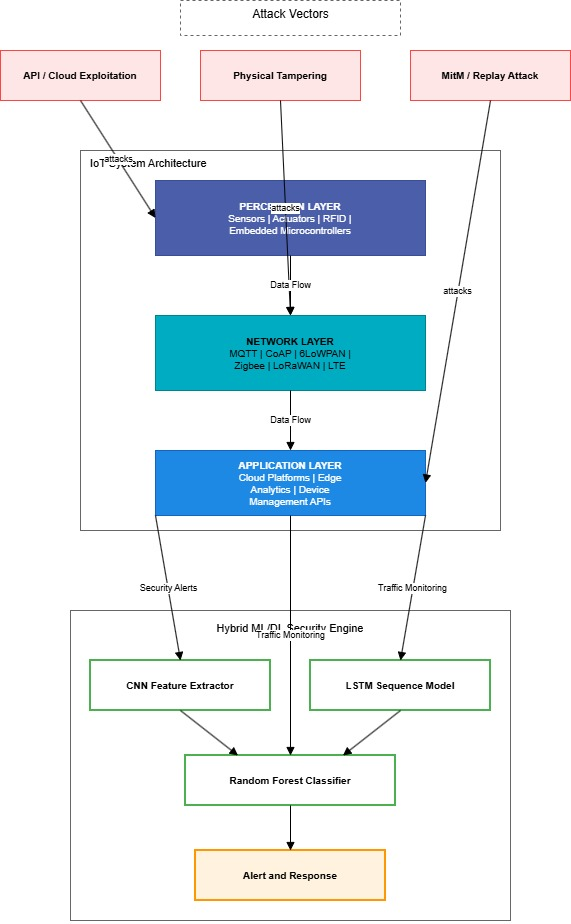
\includegraphics[width=0.50\textwidth]{figuers/fig1 (1).jpg}
    \caption{Three-tier IoT architecture illustrating the perception, network, and application layers alongside their principal attack vectors and the integration position of a hybrid machine learning and deep learning security engine. The perception layer is exposed to physical tampering, the network layer to man-in-the-middle and replay attacks, and the application layer to cloud and API exploitation. Adapted from \cite{al2015internet} and \cite{alaba2017internet}.}
    \label{fig:iot_architecture}
\end{figure}

% ---- Table 1: Concepts
\begin{table}[H]
    \centering
    \caption{Representative concepts and their technical descriptions in the context of hybrid IoT cybersecurity models. Sources: \cite{al2015internet,zhang2019hybrid,meidan2018n,ferrag2020deep}.}
    \label{tab:concepts}
    \begin{tabular}{|p{3.5cm}|p{9.5cm}|}
        \hline
        \textbf{Concept} & \textbf{Technical Description} \\
        \hline
        IoT Node &
          A resource-constrained embedded device equipped with sensing, actuation, and wireless communication capabilities, characterised by limited central processing cycles, minimal memory, and restricted energy budgets that preclude deployment of conventional security software stacks. \\
        \hline
        Intrusion Detection System &
          A monitoring component that analyses network traffic or system behaviour to identify unauthorised activities, policy violations, or ongoing cyberattacks, operating either at the network perimeter or within individual device firmware. \\
        \hline
        Feature Extraction &
          The process of transforming raw network packet captures or device telemetry streams into structured numerical representations suitable for consumption by machine learning or deep learning classification models. \\
        \hline
        Hybrid Model &
          A composite detection architecture combining two or more machine learning or deep learning algorithms to exploit complementary capabilities, achieving higher accuracy and robustness than any individual component model acting in isolation. \\
        \hline
        Federated Learning &
          A distributed training paradigm in which IoT nodes collaboratively train a shared intrusion detection model by exchanging gradient updates rather than raw traffic data, preserving device owner privacy while enabling global model improvement. \\
        \hline
        Concept Drift &
          A phenomenon in which the statistical distribution of network traffic changes over time as new devices are added or adversary tactics evolve, causing a static trained model to progressively lose predictive accuracy and require periodic retraining or online adaptation. \\
        \hline
        Anomaly Score &
          A quantitative measure produced by a detection model reflecting the degree of deviation from the learned normal behaviour distribution, with scores exceeding a calibrated threshold triggering security alerts for analyst investigation. \\
        \hline
    \end{tabular}
\end{table}


%=================================================================
\section{Core Concepts and Approaches}
%=================================================================

The process involved in the designing of the appropriate hybrid model of machine learning and deep learning approaches that can effectively be used to achieve the objective of cybersecurity for IoT devices is based on certain fundamental ideas and methods. In this section, we will discuss the key hybrid modelling techniques and architectures that have been successful in contemporary literature.

\subsection{Taxonomy of Hybrid Modelling Strategies}

Taxonomies of hybrid ML and DL models exist based on the nature of the structure among the different building blocks of such a model. This is an important consideration when choosing which architectures should be used in a particular application setting \cite{zhang2019hybrid}. The category of sequential hybrids has been the most extensively studied one to date, wherein the output of one part of the model forms the input to the other. The most common type of architecture uses a DL building block, often a CNN or RNN, to learn compact representations from traffic data followed by a traditional ML classifier to classify these features into attacks.

Parallel ensembles deploy several algorithms concurrently on the same input and aggregate the outputs using techniques like majority vote, weighted average, Bayesian aggregation, and meta-learning using stacking \cite{mirsky2018kitsune}. The reason for utilizing parallel ensembles is essentially statistical in nature. Since the aggregated outputs of various algorithms with diverse failure modes and inductive biases yield a resultant output with reduced variance compared to the constituent members, the chances of an attack vector eluding all the algorithms are greatly minimized. Parallel ensembles are especially resilient to adversarial attacks since, even if an adversary were able to generate a perturbation capable of fooling a single member algorithm, it would not be able to generate one capable of simultaneously fooling all the other member algorithms as well.

Hierarchical hybrids offer a systematic approach that incorporates decomposition, whereby high-level anomaly detection takes place using a lighter-weight algorithm on the edge devices, whereas the detected anomalies are then escalated to a heavier-weight deep learning algorithm for precise classification. The hierarchical approach is inherently suited to the resource limitations of edge IoT devices, as it is impossible to perform deep neural network inference on all packets, but entirely feasible to do so only on anomalous packets.

\subsection{CNN-Based Feature Extraction Coupled with Classical Classifiers}

One of the best-known approaches to building hybrid models for secure IoT communication is the use of CNNs for automated feature extraction, followed by classification using conventional machine learning algorithms \cite{ferrag2020deep}. In this architecture, network packet captures are preprocessed and transformed into input tensors, which are then processed by convolutional layers with rectified linear unit activation functions, along with max-pooling and batch normalization layers. Finally, a feature vector is obtained from the output of the last convolutional layer, encoding the most discriminating features of the input data, from high dimensional space to low dimensional embeddings.

It has been observed in multiple research works that such an architectural model can deliver an accuracy score that exceeds ninety-nine percent on various standard datasets such as UNSW-NB15 and NSL-KDD \cite{vinayakumar2019deep}. The benefit of this over the single deep learning model is that the ensemble method used in conjunction with a random forest classifier or a gradient boosting classifier will deliver a much more balanced probability score, lower overfitting to the peculiarities of the data distribution in the training set, and enables the decision boundary to be audited based on the feature importance score. It is worth mentioning here that the random forest model has a built-in protection against noisy or mislabeled training examples.

\subsection{LSTM-Based Temporal Modelling for Sequential Attack Detection}

Recurrent structures, especially Long Short-Term Memory structures, are well-suited to modeling temporal dependencies in network traffic flows, where complex attacks can be detected as a sequence of apparently benign actions whose purpose is malicious \cite{yin2017deep}. One login failure may not be unusual, but a series of login failures from various source IP addresses within a span of ten minutes is indicative of a credential stuffing attack. These temporal dependencies cannot be detected by stateless models, but they are exactly the type of temporal dependencies that are best modeled using Long Short-Term Memory gate units.

Long Short-Term Memory networks are usually combined with Convolutional Neural Networks in architectures where the convolutional layers learn feature representations from local regions at each timestep, while the Long Short-Term Memory layer combines these over time into a representation at the level of the entire sequence, accounting for the spatial nature of the traffic snapshots and their temporal dynamics \cite{almiani2020deep}. In experiments conducted using the CICIDS2017 dataset, hybrid CNN-LSTM networks have been shown to achieve F1-scores greater than 0.97 in several types of attacks, such as distributed denial-of-service, port scans, and web applications attacks. The results show a comparable performance to deep learning methods but with a far easier training procedure.

\subsection{Autoencoder-Ensemble Hybrids for Unsupervised Anomaly Detection}

For many IoT scenarios, labeled data pertaining to attacks may not be readily available or becomes outdated rapidly since attackers will change their attack vectors to outperform defense models that have been trained on the older attack types \cite{meidan2018n}. Autoencoders trained solely on normal traffic data capture a small manifold of normal behavior by devices. The traffic generated during an attack is abnormal and results in high reconstruction errors, thus giving us a numeric anomaly detection signal that does not require knowledge of any attacks.

Autoencoder-based hybrid models enhance this approach by training several special autoencoders that are each trained on a different dimension of the behaviour of the device, followed by using a meta-learner that learns the importance of the error from each autoencoder that is relevant for detecting anomalies in a particular kind of devices or traffic flow \cite{mirsky2018kitsune}. One such important architectural advance in the domain is the Kitsune architecture, which uses a hierarchical design of autoencoders in which several small autoencoders train independently on subsets of traffic data, and the output error from these autoencoders is used by the second-tier autoencoder to generate the final score for an anomaly. This architecture allows for online learning by adapting to changes in normal traffic patterns without having to retrain the model as a whole.


%=================================================================
\section{Comparative Discussion}
%=================================================================

An assessment of hybrid machine learning models and deep learning algorithms must be conducted by taking into consideration their position against the overall security methods, based not only on empirical results on standardized metrics but also on their applicability when dealing with specific limitations of the IoT environment. The truth is that there is no best model that excels all others in any given assessment criterion.

\subsection{Hybrid Models Versus Traditional Signature-Based Systems}

Signature-based intrusion detection systems rely on the matching of traffic observed in networks to databases that hold information about different types of attack patterns. Programs such as Snort, Suricata, and Zeek have been deployed on a larger scale than ever before, and they also have extremely low false positive rates for attacks whose variants are already well-known. However, the fact that these techniques depend completely on pre-existing knowledge means that they can never detect zero-day vulnerabilities or unknown attack variants that bear no resemblance to any attack patterns known beforehand \cite{ferrag2020deep}. Hybrid deep learning methods yield a significantly higher recall rate when dealing with attacks within novel categories than signature-based intrusion detection systems; in fact, empirical studies show that the recall rates may even be between fifteen and thirty percentage points higher in the case of zero-day attacks \cite{thamilarasu2019towards}. One disadvantage of this approach is that the false positive rate is slightly higher due to its statistical nature.

The benefit of hybrid models in terms of precision over deep learning models can be restored by including classic classifiers that are capable of training on massive labeled data sets to detect highly reliable attack signatures as opposed to anomalies. The hybrid model outperforms the individual models in a Pareto sense; it matches the recall of deep learning models but has higher precision than signature-based methods. This is the core reason why hybrid models make sense, despite the remarkable performance statistics of deep learning models, and have not been replaced by the latter models yet.

\subsection{Comparison Among Machine Learning, Deep Learning, and Hybrid Architectures}

Traditional machine learning models have proven to be highly effective at handling tabular data, scoring more than ninety-eight percent accuracy on NSL-KDD in fully supervised environments \cite{vinayakumar2019deep}. The effectiveness of traditional models decreases in line with the complexity and abstraction needed of the feature space; that is why they fail to learn from raw packet payloads due to the absence of any meaningful patterns within the feature space itself. Deep learning models can handle the challenges of high-dimensional, abstract feature spaces using learned hierarchical features, although they need much more labelled data and training capacity than traditional approaches.

Hybrid systems always offer the best possible balance among all of these criteria. They can offer equal or even greater accuracy in detection compared to the purely deep learning models, while at the same time being computationally more manageable and robust, features which are essential for efficient edge implementation \cite{hassan2020hybrid}. Pajouh et al.'s two-layer approach, including principal component analysis dimensional reduction followed by two-level classification, has demonstrated accuracy above ninety-nine percent in detecting threats in the NSL-KDD dataset, while still offering computation requirements that are in line with the limitations of embedded processors \cite{pajouh2019two}. It has been found that, when using the N-BaIoT dataset, domain-specific IoT models have significantly higher detection efficiency compared to generic IoT security models \cite{nguyen2019diot}.

\subsection{Impact of Dataset Selection on Comparative Outcomes}

The selection of the benchmark dataset has a huge impact on the performance measures that result from the use of any technique and on the comparison between competing techniques; however, this aspect is often downplayed when research papers report results using one benchmark dataset only. While the KDD Cup 1999 dataset has played a prominent role, its attack samples lack similarity to the current traffic, being easy to classify correctly and lacking the features of the current attack traffic; it cannot serve the purpose of measuring the efficiency of techniques to detect real attacks in today’s networks. In order to overcome this issue, more recent datasets such as CICIDS2017, N-BaIoT, Bot-IoT, and MQTTset were designed \cite{meidan2018n}.

Cross-dataset testing, where a detector trained on a certain dataset is tested on a different dataset coming from a different network setting, reveals consistent performance drops of more than thirty percent points, stressing the prevalence of dataset-specific overfitting problems and encouraging the study of domain adaptation methods capable of transferring learning experience across heterogeneous network settings without full re-training \cite{zhang2019hybrid}. The lesson learned here is that accuracy metrics published in scientific articles should be treated with great care unless verified with cross-dataset or deployment performance data indicating successful generalization to traffic conditions other than those of the training dataset.

% ---- Table 2: Comparison
\begin{table}[H]
    \centering
    \caption{Comparative summary of intrusion detection approaches for IoT across key evaluation dimensions under varied threat scenarios. Sources: \cite{ferrag2020deep,zhang2019hybrid,mirsky2018kitsune,vinayakumar2019deep}.}
    \label{tab:comparison}
    \begin{tabular}{|p{3.0cm}|p{2.2cm}|p{2.4cm}|p{2.3cm}|p{2.6cm}|}
        \hline
        \textbf{Approach} & \textbf{Detection Accuracy} & \textbf{Computational Cost} & \textbf{Interpretability} & \textbf{Zero-Day Detection} \\
        \hline
        Signature-Based IDS & High (known only) & Very Low & Very High & None \\
        \hline
        Classical ML (RF, SVM, k-NN) & Moderate to High & Low & High & Low \\
        \hline
        Standalone DL (CNN, LSTM) & High & High & Low & Moderate \\
        \hline
        Hybrid ML/DL & High to Very High & Moderate & Moderate & Moderate to High \\
        \hline
        Federated Hybrid Models & Moderate to High & Moderate & Low & Moderate \\
        \hline
        Autoencoder-Ensemble & Moderate & Moderate & Low & High \\
        \hline
    \end{tabular}
\end{table}


%=================================================================
\section{Practical Insights and Use Cases}
%=================================================================

Transitioning from the development stage of theoretical models to deployment stage is beset by its own unique challenges, which are often downplayed in academic analysis that concentrates solely on classification performance metrics. The following section will analyze three such scenarios where deployment of the hybrid model was successful.

\subsection{Edge Deployment and Resource Optimisation}

Machine learning and deep learning models operating at the edge of the network have become more desirable than cloud-based detection, as they significantly reduce detection-to-response time, avoid transmitting personal data contained within traffic flows, and continue to operate even when there are no connections available to the cloud, which would otherwise cause the cloud-based system to be blind \cite{thamilarasu2019towards}. The issue of resource optimization arises in this case due to the absence of floating-point processing units in edge processors, which allow deep neural networks to operate efficiently on servers.

Structured pruning of models using model compression is a technique that shrinks the model size by up to a factor of ten to fifty, with negligible accuracy losses that are well within tolerable limits for most applications of intrusion detection \cite{ge2019deep}. The pruning technique involves removing redundant synapses or feature maps whose contribution to the model performance is insignificant, thus creating a more sparse architecture with reduced multiplications and accumulation calculations during the process of inferring an output. Quantisation entails reducing the cost of parameter storage through reduced weight precision, such as using eight-bit integers instead of thirty-two-bit floats for weight parameters, making it possible to make inferences on devices without floating-point arithmetic capability.

The use of all three algorithms together in sequence has shown to result in models that can be used in devices with just one megabyte of flash memory capacity available, which makes it possible to have intrusion detection capabilities implemented directly within the device even at the lowest tier of the IoT system without relying on any edge servers or cloud services. Such an approach can provide practical benefits in cases where IoT implementations take place in remote geographical areas, where connectivity to any centralized security services is unreliable.

\subsection{Federated Learning for Privacy-Preserving Security}

Under the federated learning framework, IoT devices work together to build an intrusion detection model, whereby instead of transferring actual traffic data to the federation coordinator, they exchange only the parameter values of their models, thus ensuring that the privacy of the device owners is maintained, compliance with data privacy laws such as the General Data Protection Regulation is adhered to, and the costs associated with transmitting data to the server are minimized \cite{lyu2021towards}. In essence, each individual IoT device trains its own model parameters on the traffic it sees locally, and the only information that it shares with the federation coordinator is the gradient updates, which are then aggregated to produce a global model improvement.

Based on experimental findings, federated hybrid models are able to match the performance of the corresponding centralised models in five to ten communication rounds when working with federated datasets with balanced traffic distribution, where the observing devices in the federation see diverse samples of traffic \cite{nguyen2019diot}. The performance degradation is encountered in federations with a highly skewed traffic distribution where each device sees a very specialised type of traffic which is not representative of the overall traffic distribution. In addition, there is ongoing work being done on federated learning approaches that provide robustness to heterogeneous statistical distributions by enabling convergence in such scenarios. Another outstanding issue is how to defend against the attack where the adversary manipulates gradient updates sent by compromised devices to the fusion server.

\subsection{Integration with Security Operations Workflows}

For a hybrid machine learning/deep learning solution to offer any long-term value once deployed, it needs to be able to work in conjunction with Security Information and Event Management (SIEM) tools and generate meaningful outputs that assist human decision-making without creating an alerting overload problem that results in alert fatigue \cite{ferrag2020deep}. A key task for the classification process is thus to take a probability distribution generated by the classifier and transform it into an informative SIEM alert object that includes not only the decision itself but also its rationale expressed in terms understandable to non-experts in machine learning.

Techniques for explainable artificial intelligence like SHAP values and LIME offer post-processing explanations highlighting which inputs were most responsible for a particular detection, thereby allowing analysts to determine the validity of a detection and allocate their attention resources to only the most convincing malicious activities \cite{xiao2019iot}. The adoption of hybrid explainability solutions within security operations centers has been found to yield substantial gains in mean time to investigation and analyst confidence in automated detection outcomes, tackling the previous reluctance of security practitioners to act on detections made using black-box systems. Beyond the technical implementation of explainable artificial intelligence, the operational integration process involves determining a strategy for sorting out confident detections for automated handling and uncertain alerts for human review.


%=================================================================
\section{Challenges and Open Issues}
%=================================================================

While much has been achieved in terms of hybrid machine learning and deep learning-based IoT security, many issues still need to be sorted out in various respects. It is crucial to know about these issues to be able to separate minor improvements in IoT security from real obstacles to the actual use of these technologies in production settings.

One of the biggest technical challenges that concept drift poses to the viability of long-term deployment is the issue of concept drift itself \cite{xiao2019iot}. The models built using past traffic data increasingly diverge from the current traffic distributions due to the introduction of new devices, firmware updates, shifts in application behavior, and changes in adversary behavior designed to evade existing detection systems. Without regular retraining or adaptation, models will have an ever-increasing rate of false negatives as the divergence between the training distribution and current distribution increases. One way to address this is through full retraining, but this comes with both a cost in terms of operational complexity and a window of vulnerability to attacks when transitioning. An alternative approach involves online adaptation, which continually modifies the model using live data without relying on retraining, but this brings its own problems of stability and robustness to adversarial tampering.

The notion of adversarial robustness is highly relevant and has been a subject of extensive investigation following the revelation that deep neural networks are vulnerable to attacks that result in systematic misclassification caused by perturbations that are indistinguishable from genuine data to humans \cite{vinayakumar2019deep}. Within the context of cybersecurity, an attacker familiar with the adopted detection system could design network traffic whose statistical features match those of benign traffic, while its semantics correspond to that of an attack. While certified robustness verification techniques offer strong guarantees about the properties of a trained model within a perturbation region, they are computationally expensive and currently only support simplistic model designs.

Constraints on data quality and availability have a distinct impact on all phases of developing ML and DL solutions specifically within the domain of IoT security. Imbalanced data sets characterized by extreme class imbalance, where attack traffic represents only one percent of all traffic analyzed and labeled, make oversampling approaches crucial to training ML models \cite{pajouh2019two}. This can be achieved using approaches such as the Synthetic Minority Over-sampling Technique (SMOTE) or Generative Adversarial Network (GAN)-based approaches. Privacy concerns and legal regulations create another set of challenges, as analyzing network traffic includes inspecting communications which might fall under the scope of data protection legislation like the General Data Protection Regulation (GDPR) of the European Union or the California Consumer Privacy Act (CCPA) in the USA. Consequently, these legal regulations constrain the datasets available for training as well as traffic available for testing of developed models and introduce legal challenges that need to be addressed when developing ML-based solutions in the domain of IoT security.

Heterogeneity of the mixed devices in an IoT environment is a modelling problem without any solution in existing studies. A healthcare IoT system can have several kinds of devices including radiology machines, monitoring tools, computers in office, building control devices and WiFi nodes for visitors, and the statistics associated with the traffic produced by each kind of devices is different from each other. In the case of applying one universal model to detect anomalies in mixed traffic data, performance of the model will suffer in the cases where some kind of devices is statistically underrepresented in the dataset \cite{alaba2017internet}.


%=================================================================
\section{Future Directions}
%=================================================================

The path to future development in hybrid machine learning and deep learning algorithms for IoT cybersecurity leads to multiple emerging areas of study in wireless networks, autonomous devices, cloud computing, and artificial intelligence which have already started being applied, and which will shape the field over the next ten years \cite{zhang2019hybrid}.

There seems to be much promise in using transfer learning and domain adaptation techniques in mitigating the current generalization problems faced by hybrid intrusion detection systems. Through transfer learning, which involves first training the hybrid model on a big dataset covering a wide range of device classifications, network configurations, and threat classes, followed by the fine-tuning of the same model based on small amounts of local data to suit particular contexts, the costs and time involved in making security measures operational in newly encountered environments can greatly be minimized \cite{thamilarasu2019towards}. Given that transfer learning is founded on the idea that learning representations acquired in a particular task/domain will make it easier to learn in another similar task/domain, its application in network security is quite logical, especially because attack methods share similar low-level statistics irrespective of the differences in network devices and applications.

Integrating the ideas from large language models into the field of IoT security analysis is one such frontier that promises to revolutionize the way we reason about cyber threats. The use of foundation models trained on telemetry data sets such as intrusion detection logs, vulnerability databases, incidents, and traffic capture information allows us to create universal security reasoning engines capable of quickly learning how to analyze new types of threats using few-shot prompting without fine-tuning for domain-specific security concepts \cite{lyu2021towards}. While the computational cost of inference from large language models means that they cannot be deployed directly on IoT devices, the model reduction techniques discussed in Section 5 offer promise of creating smaller-sized security models capable of reasoning about wide ranges of cyber attacks like their full-size counterparts.

The neuromorphic computing architecture with spiking neural networks is an entirely different approach to computation that uses significantly lower amounts of power compared to the traditional von Neumann architecture, making possible continuous real-time inference on IoT battery-powered devices without the energy budget required by traditional deep learning inference \cite{xiao2019iot}. Spiking neural networks operate based on spike train encoding of information that fits naturally into the problem of analysis of network traffic events in that the vast majority of the time steps do not contain any information related to attacks. The early results with intrusion detection systems using spiking neural networks show promise in performance comparable to conventional deep learning solutions; however, the training techniques are still somewhat immature compared to those used for conventional deep learning.

The ability to develop collaborative threat intelligence sharing platforms using secure multi-party computation and homomorphic encryption is another important organisational step forward alongside the technological achievements described above \cite{nguyen2019diot}. Each IoT installation captures only a limited portion of the threat landscape, and any model created based on that data is only capable of responding to the attacks that were conducted against it. Being able to share information about attacks in such a way that the underlying statistical properties can be used without revealing any potentially compromising operational details will allow all parties involved to leverage the threat detection expertise of the entire community, thus speeding up the adaptation process of already installed models. The necessary cryptographic mechanisms are already sufficiently developed within the scientific community and ready for prototyping, although some open issues still exist in terms of standardization and governance of threat intelligence sharing communities.


%=================================================================
\section{Conclusion}
%=================================================================

The development of hybrid ML/DL architectures for the cyber security of the IoT has advanced considerably from being a process of merely adapting general-purpose intrusion detection algorithms to an applied science based on the unique technical properties of adversarial, heterogenous, and resource constrained IoT environments. The paper has explored the subject starting with its foundational elements in terms of the IoT architectural design and threats, continuing with the discussion of current approaches to modelling hybrid architectures and their particular implementations, and concluding with current implementation and research problems.

The first main conclusion drawn from the comparative analysis is that there is no one-size-fits-all detection architecture that will perform well under all operational settings, threat types, and limitations on computational resources. Signature-based techniques yield very high precision in the detection of known attacks at low computational overhead costs but lack the capability to detect any new variations of attacks, even zero-day attacks. Deep learning models yield excellent results in terms of raw performance, but they demand computational costs beyond what edge IoT devices can handle, and their outputs cannot be easily interpreted. The most promising solution currently available is hybrid architectures that incorporate both deep learning of features and classical classifiers, which balance all desirable factors.

These open problems identified in this article, namely concept drift in sustainable deployment, robustness to adaptive adversaries, constraints of data quality and class imbalance, and heterogeneity across mixed devices in real-world IoT applications, cannot be addressed as mere optimization issues. These are the key gaps that separate the findings in experimental benchmarks from the reality of deploying solutions that improve security on an urban and industrial scale. Closing these gaps demands concerted effort among the communities of machine learning, network security, system engineering, hardware design, privacy law, and policymaking.

The external environment in which this progress will take place is characterized by the increasing deployment of fifth- and future sixth-generation cellular networking capabilities, which offer sub-millisecond network latency for IoT edge connectivity, the widespread adoption of interconnected and semi-autonomous devices, the rapid evolution of neuromorphic and quantum computing architectures, and increasingly sophisticated management frameworks for smart cities which create the context for advanced IoT security solutions \cite{khan2018iot}. Those organizations which are able to implement a hybrid intelligence-based approach to their IoT security requirements will be able to enjoy significant benefits in terms of the scope of threat detection, robustness of operation, and compliance with the increasingly stringent regulatory environment regarding data protection issues. The technology is mature enough to facilitate this process, and all that is required now is the engineering expertise and institutional commitment to making it happen.


\bibliographystyle{plain}
\bibliography{references}

\end{document}
